
\chapter{Présentation}
\label{chapter:poodlePres}

L'attaque Poodle (Padding Oracle On Downgraded Legacy Encryption)

a été découverte par Bodo Möller, Thai Duong et 
Krzysztof Kotowicz\cite{article:ssl-poodle} en septembre 2014.\\

Cette attaque se base sur une faiblesse de SSLv3.
Elle fonctionne pourtant sur les dernières versions de TLS.
Pour maintenir la compatibilité avec tout les clients, un
serveur TLS peut rétrograder en version SSLv3.\\

C'est une attaque de typer Man-In-The-Middle (l'homme du milieu).
L'attaquant peut utiliser un site malveillant qui injecte un
code javascript sur le client pour le faire générer des requêtes
sur le serveur cible. Il peut alors forcer l'utilisation de 
SSLv3, même si le client et le serveur utilisent TLS.\\

L'objectif de l'attaque est de voler le cookie de session 
du client. Pour cela, comme BEAST, l'attaquant force 
l'utilisation du mode CBC. Elle utilise le \emph{padding oracle attack }

\chapter{Mise en place de l'attaque}
\label{chapter:Poodleattack}

\section{Packet SSL}
\label{sec:packet}

Le Format des paquets SSL est le suivant : 

\begin{figure}[h]
  \centering
  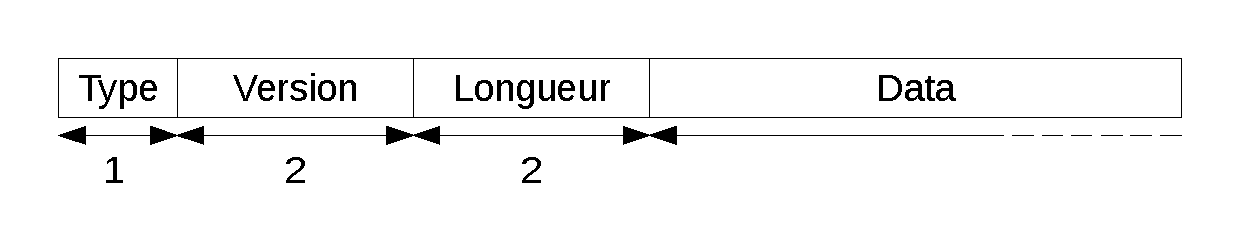
\includegraphics[scale=0.5]{schemaSSL.pdf}
  \caption{Schéma d'un paquet SSL}
  \label{fig:ssl}
\end{figure}


Type :
\begin{itemize}
\item 0x16 : Handshake
\item 0x14 : Change Cypher Spec
\item 0x15 : Alert
\item 0x17 Application Data
\end{itemize}

Version :
\begin{itemize}
\item 0x3000 : SSLv3
\item 0x30xy : TLSvx.y
\end{itemize}

Les données sont chiffrées et leurs tailles est indiquées par
la longueur.

\section{Man In The Middle}
\label{sec:mitm}

\section{Injection de Code}
\label{sec:injCode}





